\chapter{Environnement et application}
\label{ch:app}

Nous allons aborder, dans ce chapitre, le nouvel environnement créé à l'aide de Docker et le nouveau code produit à partir de celui de la thèse \thLeite.

L'environnement est réalisé à l'aide de \emph{Docker Compose}, il est composé de trois images différentes. Le code, orienté objet sera exécuté dans ce nouvel environnement.

\section{Images Docker}
Tous les fichiers nécessaires à la construction des images de notre environnement se trouvent dans le dossier \emph{$developpement/dockers$}.

\subsection{Hmmer}
La première image est celle visant à remplacer l'utilisation de l'\gls{api} en ligne de HMMER. Il s’agit d'encapsuler l'application HMMER afin de pouvoir l'utiliser pour traiter les séquences protéiniques.

Les fichiers nécessaires se trouvent dans le dossier \emph{$developpement/dockers/hmmer$}. Il s’agit d'une image basée sur \emph{centos}, qui est une image de base Docker très légère.

Tout d'abord, le \emph{Dockerfile} de cette image installe le compilateur C++ \emph{gcc}. Puis, il récupère les sources de l'application HMMER et les compile.

Pour davantage de détails, veuillez consulter directement le fichier \emph{Dockerfile} de l'image.

\subsection{Database}
L'application nécessite plusieurs bases de données Mysql. L'image \emph{database}, dont les sources se trouvent dans le dossier \emph{$developpement/dockers/database$}, remplit cette fonctionnalité.

Pour des raisons de simplicité, cette image est construite à partir de Debian Jessie, la différence entre Centos et Debian est négligeable du fait que nous ne lancerons qu'un seul conteneur de cette image.

Dû à la fois à la phase de débug et pour de futurs débugs, l'image est construite avec un certain nombre de paquets afin de faciliter la vie du développeur.

La mise en place d'une image \emph{Docker} avec un serveur mysql n'est, par expérience, jamais une chose facile à réaliser. C'est pour cela que nous allons entrer un peu plus dans les détails des différentes commandes qui composent le fichier \emph{Dockerfile} de cette image. Il n'est pas forcément nécessaire de lire ce sous-chapitre pour comprendre les aboutissants de cette thèse, mais il est nécessaire que les informations qui suivent y figurent.

Premièrement, afin de pouvoir accéder au conteneur lancé à partir de cette image, il faut faire en sorte que mysql écoute les connexions en entrée.

\lstset{language=bash}

\begin{lstlisting}[frame=single]
RUN sed -i -e"s/^bind-address\s*=\s*127.0.0.1/bind-address = 0.0.0.0/" /etc/mysql/my.cnf
\end{lstlisting}

Maintenant que notre conteneur peut recevoir des connexions, on installe \emph{mysql-server mysql-client libmysqlclient-dev} qui installent Mysql sur notre image.

On peut démarrer le service Mysql:

\begin{lstlisting}[frame=single]
RUN mysqld &
RUN service mysql start
\end{lstlisting}

On n’oublie pas d'exposer le port de connexion que l'on souhaite. Ici le 3306 qui est le port par défaut de Mysql.

\begin{lstlisting}[frame=single]
EXPOSE 3306
\end{lstlisting}

On modifie également quelques configurations Mysql, afin de pouvoir utiliser des fichiers \emph{.sql} de tailles plus grandes.

\begin{lstlisting}[frame=single]
RUN sed -ire 's/max_allowed_packet.*=.*/max_allowed_packet = 200M/g' /etc/mysql/my.cnf
RUN sed -ire 's/key_buffer_size.*=.*/key_buffer_size = 128M/g' /etc/mysql/my.cnf
\end{lstlisting}

On ajoute le fichier \emph{startup.sh} et on fixe qu'au lancement du conteneur il soit exécuté.

\begin{lstlisting}[frame=single]
ADD ./startup.sh /opt/startup.sh

CMD ["/bin/bash", "/opt/startup.sh"]
\end{lstlisting}

Regardons ce que l'on trouve dans le fichier \emph{startup.sh}:

\begin{figure}[H] 
\centering 
\begin{lstlisting}[frame=single]

if [ ! -f /var/lib/mysql/ibdata1 ]; then

	mysql_install_db

	/usr/bin/mysqld_safe &
	sleep 10s

	echo "GRANT ALL ON *.* TO admin@'%' IDENTIFIED BY 'root' WITH GRANT OPTION; FLUSH PRIVILEGES" | mysql

	# For 1_F1 DetectDomains.py
	echo "CREATE DATABASE phage_bact" | mysql
	mysql phage_bact < /tmp/db/phagesVD.sql
	mysql phage_bact < /tmp/db/bacteriaVD.sql
	mysql phage_bact < /tmp/db/interactionsVD.sql
	mysql phage_bact < /tmp/db/neg_interactionsVD.sql
	mysql phage_bact < /tmp/db/protdom_create.sql
	mysql phage_bact < /tmp/db/progress_create.sql
	mysql phage_bact < /tmp/db/progress_interaction_create.sql

    # For 3_F1 countScoreInteraction.py
	mysql phage_bact < /tmp/db/score_interactions_create.sql

	echo "CREATE DATABASE domine" | mysql
    mysql domine < /tmp/db/domTGo.sql
    mysql domine < /tmp/db/domPfam.sql
    mysql domine < /tmp/db/domPgmap.sql
    mysql domine < /tmp/db/domTInteract.sql

    # For 4_F1 FreqQtdScores.py
	mysql phage_bact < /tmp/db/qtd_scores_create.sql

	killall mysqld
	sleep 10s
fi

/usr/bin/mysqld_safe
\end{lstlisting}
\caption[Création bases de données]{Création bases de données}
\label{fig:createDb} 
\end{figure}

Dans ce script, on commence par donner les privilèges Mysql à l'utilisateur admin. Ensuite on met en place les différentes bases de données, \emph{$phage_bact, domine$}, dont l'application a besoin. On crée ces deux bases de données et leurs tables.

Dans l'éventualité où l'on souhaiterait ajouter une nouvelle base de données, c'est ici qu'il faudra ajouter la commande Mysql de création.

De plus si l'on souhaite ajouter des tables ou données à une de nos bases de données, c'est également dans ce fichier qu'il faudra le faire.

Comme vous pouvez le voir, tous les fichiers \emph{.sql} nécessaires sont placés dans le dossier \emph{$developpement/dockers/database/data$}.


\subsection{Core}
Dû à la fois à la phase de débug et pour de futurs débugs, l'image est construite avec un certain nombre de paquets afin de faciliter la vie du développeur.

C'est véritablement cette image qui contient tout ce qui est nécessaire à l'exécution de l'aspect bio-informatique de l'application. C'est également elle qui contrôle l'application, étant donné que c’est dans ce conteneur que le code de l'application est exécuté.

Comme pour l'image \emph{database} on installe les paquets nécessaires à utiliser Mysql, \emph{mysql-server, mysql-client, libmysqlclient-dev} et python.

On installe pip3, le gestionnaire de paquets pip pour python3:

\begin{figure}[H] 
\centering 
\begin{lstlisting}[frame=single]
RUN apt-get install -y python3-pip r-base
\end{lstlisting}

On installe aussi un des paquets les plus importants de cette image.

\begin{lstlisting}[frame=single]
RUN pip3 install biopython
\end{lstlisting}

Afin d'accéder à la base de données depuis le code python il nous faut installer le paquet:

\begin{lstlisting}[frame=single]
RUN pip install mysql-connector
\end{lstlisting}

Finalement, on installe Docker, car il nous faudra pouvoir communiquer avec l'engin Docker de l'hôte, afin d'exécuter des conteneurs de l'image HMMER.

\begin{lstlisting}[frame=single]
RUN apt-get install -y curl
RUN curl -fsSL https://get.docker.com/ | sh
\end{lstlisting}
\caption[Core installations]{Core installations}
\label{fig:coreInstall} 
\end{figure}

\section{Docker Compose}
Maintenant que nous avons toutes les images nécessaires à notre environnement applicatif orienté bioinformatique, nous allons voir comment les combiner à l'aide de \emph{Docker Compose}.

La figure \ref{fig:architecture} montre l'architecture qui est mise en place à l'aide de \emph{Docker}.

\begin{figure}[H] 
\centering 
\includegraphics[width=0.7\columnwidth]{img/architecture} 
\caption[architecture]{Architecture de l'environnement}
\label{fig:architecture} 
\end{figure}

La figure \ref{fig:architecture} montre qu'un conteneur construit à partir de l'image \emph{Core} contrôlera l'exécution du code applicatif et la création de conteneurs basés sur l'image \emph{hmmer}. De plus, tout ce qui a trait aux données stockées en SQL sera géré par le conteneur \emph{Database}.

De cette manière, le conteneur \emph{Core} peut créer des conteneurs \emph{hmmer} pour exécuter les recherches de domaines protéiniques.

Regardons comment cela est mis en place grâce à \emph{Docker Compose}. 

Premièrement, il nous faut un service qui lancera notre conteneur de base de données:

\begin{figure}[H] 
\centering 
\begin{lstlisting}[frame=single]
database:
    build: ../dockers/database
    tty: true
    environment:
      MYSQL_ROOT_PASSWORD: SecretPasswordInphinity
      MYSQL_USER: inphinity
      MYSQL_PASSWORD: SecretPasswordInphinity
      MYSQL_DATABASE: phage_bact
    ports:
      - 3309:3306
    networks:
      mynet:
        ipv4_address: 172.25.0.102
    container_name: inphinity-database
    volumes:
      - /inphinity-data/mysql:/var/lib/mysql
\end{lstlisting}
\caption[Service base de données]{Service base de données}
\label{fig:serviceDb} 
\end{figure}

On spécifie que l'on souhaite construire notre conteneur à partir de l'image se trouvant dans le dossier \emph{$/dockers/database$}. En effet, à l'exécution de la commande de lancement de notre \emph{compose}, docker compose construira l'image \emph{Database} et créera un conteneur à partir de cette image.

On fixe les paramètres de configuration de Mysql, tels que le mot de passe root, l'utilisateur, son mot de passe et le nom de la base de données par défaut.

On route les ports utiles au conteneur, ainsi que le réseau virtuel qui sera utilisé.

On fixe manuellement le nom du conteneur qui sera créé afin de facilement pouvoir y accéder en cas de besoin (debug, tests, etc.).

Finalement, on ajoute les volumes que l'on souhaite à notre conteneur. En effet, avec cette dernière commande, on attache le dossier hôte \emph{$/inphinity-data/mysql$} au dossier \emph{$/var/lib/mysql$} du conteneur. De cette manière lorsque l'on arrête et relance notre application notre base de données ne sera pas détruite. Si l'on souhaite supprimer la base de données et en recréer une vierge, il suffit de supprimer le contenu du dossier \emph{$/inphinity-data/mysql$}.

Deuxièmement, il nous faut un service qui lancera le conteneur de notre contrôleur:

\begin{figure}[H] 
\centering 
\begin{lstlisting}[frame=single]
core:
    build: ../dockers/core
    hostname: core
    networks:
      mynet:
        ipv4_address: 172.25.0.101
    tty: true
    volumes:
      - ../inphinity:/inphinity:Z
      - ../dockers/core/data-hmm:/data-hmm:Z
      - /var/run/docker.sock:/var/run/docker.sock
    privileged: true
    links:
      - database:database
    depends_on:
      - database
    container_name: inphinity-core
\end{lstlisting}
\caption[Service contrôleur]{Service contrôleur}
\label{fig:serviceCore} 
\end{figure}

On suit exactement la même logique que pour notre premier service. On spécifie que l'on souhaite construire notre conteneur à partir de l'image se trouvant dans le dossier \emph{$/dockers/core$}. En effet, à l'exécution de la commande de lancement de notre \emph{compose}, docker compose construira l'image \emph{Core} et créera un conteneur à partir de cette image.

On attribue le réseau virtuel qui sera utilisé, le même que pour le service de la base de données.

On fixe manuellement le nom du conteneur qui sera créé, afin de facilement pouvoir y accéder en cas de besoin (debug, tests, etc.).

On ajoute les volumes nécessaires:

\begin{itemize}
\item ../inphinity:/inphinity, contient le code applicatif;
\item ../dockers/core/data-hmm:/data-hmm, servira à transmettre les fichiers de résultats des analyses réalisés par les conteneurs hmmer au contrôleur;
\item /var/run/docker.sock:/var/run/docker.sock, permet au contrôleur de communiquer avec l'engin Docker de l'hôte et donc de créer les conteneurs hmmer à la volée.
\end{itemize}

On lie, grâce à la commande \emph{links}, le contrôleur à la base de données.

La commande \emph{$depends_on$} permet de garantir que le conteneur "core" sera créé uniquement après la création du conteneur "database".

Le troisième service se trouvant dans le fichier compose n'est pas nécessaire, car on lancera les conteneurs hmmer directement depuis le code python de notre application. 

Finalement, on définit un réseau dans lequel on place les conteneurs de l'application.

\section{<<Inphinity Environment>>}

Comme déjà précisé précédemment, une première optimisation du code est passée par le fait de traduire les codes existants du python2 vers le python3.3 .

Au niveau du code, la logique suivie a été de diviser le code en \emph{phases} successives. Chacune de ces phases est chargée d'un traitement spécifique de remplir un objectif.

Attention, ce chapitre n'aborde pas la logique du code réalisé dans la thèse \thLeite , il n'est question ici que de la plus-value ajoutée lors de ce travail de master.

Les fonctions utilisées dans les scripts de la thèse \thLeite restent très proches de celle de ce travail!

\subsection{Diagramme de classes}
\begin{figure}[H] 
\centering 
\includegraphics[width=1\columnwidth]{img/class_diagram} 
\caption[classdiagram]{Diagramme de classes}
\label{fig:classdiagram} 
\end{figure}

\subsubsection{Core}
La classe \emph{Core} est la classe principale de l'application. C'est elle qui est chargée d'instancier les classes nécessaires au bon déroulement du code et de lancer les phases du processus.

Comme on le voit sur la figure \ref{fig:classdiagram}, la classe \emph{Core} possède une instance des cinq classes, représentant chacune une phase du processus. Elle possède également une instance de la classe \emph{Tools}, qui donne accès à l'objet de la classe \emph{Config}, gérant le \emph{parsing} de la configuration en cours. De plus, la classe \emph{Tools} possède un accès à l'objet \emph{DBUtilities}, qui gère l'ensemble des accès aux bases de données.

\subsubsection{Phase 1 - DetectDomaines}

C'est durant cette phase que l'utilisation à HMMER est faite, c'est dans cette phase que la parallélisation de cette utilisation est réalisée. Plus précisément regardons la fonction \emph{$seek_domaines_multiprocess()$}, on y initialise une \emph{Multiprocessing.Pool} avec un certain nombre de coeurs à disposition. Ce nombre de coeurs est défini dans les fichiers de configuration, cf. \ref{ch:config}.

Ensuite, on divise le tableau des séquences à traiter en \emph{chunk}, cela permet d'obtenir les résultats également par séries de 'n' réponse et de les incérer dans la base de données au fur et à mesure. Cela afin d'éviter de perdre du temps d'analyse en cas d'arrêté de l'application.

\begin{figure}[H] 
\centering 
\lstset{language=python}
\begin{lstlisting}[frame=single]
chunk_size = pool_size * self.tools.configuration.get_chunk_size_multiplier()
        chunks = self.chunks(list(tab), chunk_size)
\end{lstlisting} 
\caption[Processus pool]{Processus pool}
\label{fig:processPool} 
\end{figure}

Lorsque l'on insère les résultats dans la base de données on insère également dans la table \emph{progress} quelles séquences ont été analysées. Cela nous permet d'arrêter et de relancer l'application quand on veut sans pour autant devoir recommencer la phase d'analyse a zéro.

On exécute le code suivant pour chacun des \emph{chunks}:

\begin{figure}[H] 
\centering 
\begin{lstlisting}[frame=single]
for chunk in chunks:
            print('%d sequences processed!' % total_processed)
            LOGGER.log_normal('%d sequences processed!' % total_processed)
            total_processed += chunk_size
            results = p.map(self.hmmer_scan.analyze_domaines, chunk)
            print(results)

            for prot in chunk:
                self.tools.db.analyze_done(prot[0], 1)

            for result in results:
                try:
                    id_prot = result[0]
                    domaines_returned = result[1]

                    self.tools.db.execute_insert_domains(id_prot, domaines_returned, id_cell, bool_bacteria, "--")
\end{lstlisting} 
\caption[Division en Chunks]{Division en Chunks}
\label{fig:chunks} 
\end{figure}

On fait appel de manière parallèle à la fonction \emph{$hmmerScan.analyze_domaines()$}. Grâce à la \emph{pool} de processus la fonction sera exécutée simultanément un certain nombre de fois.

Allons voir plus en détails ce qui se passe dans cette fonction. Pour voir le code de la fonction en détails, veuillez vous rendre directement dans les sources du code (\emph{$developpement/inphinity/v_0.5/hmmerScan.py$}).

La séquence envoyée à la fonction est \emph{parsée} dans un fichier temporaire:

\begin{lstlisting}[frame=single]
fasta = '>' + values_tab[0] + '\n' + values_tab[1] + '\n'
fasta_filename = '/data-hmm/tmp/' + str(uuid.uuid4()) + '.fasta'
self.io.write(fasta_filename, fasta)
\end{lstlisting} 

On crée également un fichier temporaire où sera stocké le résultat de l'analyse par \emph{HMMER scan}:

\begin{lstlisting}[frame=single]
results_filename = "/data-hmm/results/hits_test_" + str(uuid.uuid4()) + ".txt"
\end{lstlisting} 

Par la suite le code fait appel à la fonction \emph{Subprocess.Popen()} permettant de réaliser de commande UNIX directement depuis un code Python. Grâce à cela on peut lancer une commande qui créera un nouveau conteneur Docker qui effectuera une analyse de séquence, une fois l'analyse effectuée le conteneur s'arrête automatiquement.


\begin{figure}[H] 
\centering 
\begin{lstlisting}[frame=single]
p = subprocess.Popen([
                "docker " +
                "run " +
                "--rm " +
                "--privileged " +
                "-v " +
                path_to_core + "/data-hmm:/data-hmm " +
                "inphinity-hmmer " +
                "hmmsearch " +
                "--tblout " +
                results_filename + " " +
                "/data-hmm/Pfam-A.hmm " +
                fasta_filename
            ], stdout=subprocess.PIPE, shell=True)

            (output, err) = p.communicate()

            # This makes the wait possible
            p_status = p.wait()
\end{lstlisting} 
\caption[Popen Docker Hmmer]{Popen Docker Hmmer}
\label{fig:popenHmmer} 
\end{figure}

Cette commande lance un conteneur docker avec l'image que l'on a préalablement créée pour encapsuler HMMER. On spécifie le fichier dans lequel se trouve la séquence au format \emph{FASTA}, ainsi que le fichier dans lequel on souhaite inscrire les résultats de l'analyse.

Ensuite, on lit, récupère et filtre les résultats:

\begin{lstlisting}[frame=single]
results = self.io.read_results(results_filename, self.configuration.get_detailed_logs())

[...]
\end{lstlisting}

Nous aborderons la sélection des résultats dans la section \ref{ch:config}.

Finalement on supprime les deux fichiers temporaires et  retourne les résultats.

\begin{figure}[H] 
\centering 
\begin{lstlisting}[frame=single]
p = subprocess.Popen([
	"rm",
	results_filename
 ])
 p.communicate()
 p_status = p.wait()

 p = subprocess.Popen([
 	"rm",
 	fasta_filename
 ])
 p.communicate()
 p_status = p.wait()

return [values_tab[0], returned_domains, [start_time, end_time]]
\end{lstlisting}
\caption[Popen remove]{Popen}
\label{fig:popen} 
\end{figure}

\subsection{Configuration}
\label{ch:config}

Toutes les interactions utilisateurs que les scripts produisent lors de la thèse \thLeite ont été remplacées par une valeur dans le fichier de configuration.

\subsubsection{Lancement des configurations}

La classe \emph{Main} de l'application (app.py) est faite pour lancer la fonction \emph{$Core.run()$} pour chaque fichier de configuration se trouvant dans le dossier \emph{$inphinity/v_0.5/configs$}. Il faut préciser que seuls les fichiers finissant par l'extension \emph{.ini} sont considérés comme des fichiers de configuration. Donc pour garder une configuration, tout en empêchant qu'elle soit utilisée, il suffit d'ajouter \emph{.old} à la fin, par exemple.

\begin{figure}[H] 
\centering 
\begin{lstlisting}[frame=single]
if __name__ == '__main__':
    os.chdir("inphinity/v_0.5/configs")
    configs = glob.glob("*.ini")

    for config_file in configs:
        print('Config file: %s' % config_file)

        c = Core(config_file)
        c.run()
\end{lstlisting}
\caption[Main]{Main}
\label{fig:main} 
\end{figure}

Voici un fichier de configuration standard:

\begin{figure}[H] 
\centering 
\begin{lstlisting}[frame=single]
[INFORMATION]
verbose = 0
detailed_logs = 0
testing = 0
[ENV]
path_to_core = /home/kamyh/projects/master/developpement/dockers/core
#Dile to parse sequences
temp_file_pseqs = /tmp/tmpMF.txt
reset_db_at_start = 0
#if = 0 --> auto
#if = -1 --> nbr of core
#if = x --> x
process = -1
# Smaller the chunk are, the more time is lost
chunk_size_multiplier = 4
phases_to_run = 1,2,3,4,5
[PHASE_1]
analyze_phage = 1
analyze_bacteria = 1
[DOMS_SELECTION]
use_e_value_selection = 0
min_e_value = 9.8e-25
max_e_value = 1500

use_score_selection = 0
min_score = 0
max_score = 1500

use_biais_selection = 0
min_biais = 0
max_biais = 1500
[DATASET_GENERATION]
grades_file_pseqs = /inphinity/grades/gradesDict.p
ds_dir = /inphinity/datasets/
normalisation = 0
# 1 --> Number of bins
# 2 --> Vector of bins
type_bins = 1
number_of_bins = 1
space_between_bins = 1
\end{lstlisting}
\caption[Fichier de configuration]{Fichier de configuration}
\label{fig:configFile} 
\end{figure}

Étant donné l'importance des fichiers de configuration dans la production de dataset intéressants, nous allons passer en revue les différents éléments y étant définis.

Premièrement, il faut savoir que l'on trouve deux types d'éléments dans un fichier de configuration, des sections et de valeurs. Les sections sont des mots clés entre crochets, eg. [INFORMATION], et en majuscules. Les valeurs sont en minuscules, et se rapportent chacune à une section. En effet, toutes les valeurs après une section font partie de cette section. Cela permet d'organiser le fichier de configuration au mieux.

\textbf{Section - [INFORMATION]}

Ces valeurs de configuration servent lors des phases de développement et tests.

\begin{itemize}
\item \emph{verbose}, permet de désactiver la plupart des affichages console.
\item \emph{$detailed\_logs$}, permet d'inscrire dans les logs des informations détaillées sur l'exécution de l'application.
\item \emph{testing}, permet de limiter le nombre d'organismes traités par l'application, à des fins de développement ou de tests. 
\end{itemize}

\textbf{Section - [ENV]}

Les configurations se trouvant sous cette section concernent des variables d'environnement de l'application.

\begin{itemize}
\item \emph{$path\_to\_core$}, afin de fonctionner, l'application a besoin de connaitre l'emplacement du dossier contenant la description Docker de l'image du contrôleur principal.
\item \emph{$temp\_file\_pseqs$}, permet de spécifier le fichier temporaire qui sera utilisé afin de parser les séquences multi-fasta. 
\item \emph{$reset\_db\_at\_start$}, permet de réinitialiser la base de données au lancement de l'application.
\item \emph{process}, spécifie le nombre de coeurs qui sera alloué à la \emph{pool}. 
\begin{itemize}
\item fixé à "0", laisse la librairie automatiquement définir le nombre de coeurs, normalement le nombre maximum disponible.
\item fixé à "-1", fixe le nombre de coeurs au maximum disponible moins 1. Cette méthode permet de laisser un coeur libre pour les processus de la machine hôte.
\item fixé à "x", laisse choisir le nombre de coeurs, mais attention, en mettre davantage que le maximum ralentit l'exécution de l'application.
\end{itemize}
\item \emph{$chunk\_size\_multiplier$}, définit la taille de \emph{chunk} pour le traitement des séquences lors de la phase 1.
\item \emph{$phases\_to\_run$}, permet de définir quelles phases on souhaite exécuter. Par exemple, si la valeur est égale à "1,2,3,4,5", toutes les phases seront exécutées. On peut choisir de n'exécuter que les deux dernières phases en inscrivant la valeur de ce paramètre à "4,5".
\end{itemize}

\textbf{Section - [$PHASE_1$]}

Configurations se rapportant directement à l'exécution de la phase 1 du traitement.

\begin{itemize}
\item \emph{$analyze\_phage$}, permet de définir si les phages doivent être traités.
\item \emph{$analyze\_bacteria$}, permet de définir si les bactéries doivent être traitése.
\end{itemize}

\textbf{Section - [$DOMS\_SELECTION$]}

Une analyse de séquence par \emph{hmmsearch} donne des résultats semblables à la figure \ref{fig:hmmseach}. On voit que chaque domaine trouvé possède une valeur de score, une e-value et un biais.

\begin{figure}[H] 
\centering 
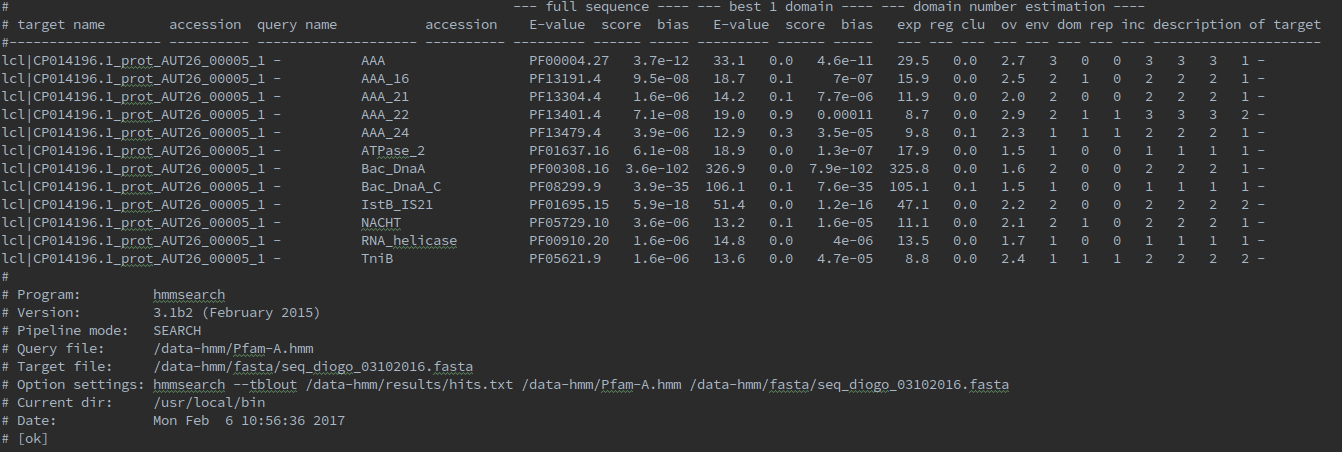
\includegraphics[width=1\columnwidth]{img/hmmsearchresult} 
\caption[hmmseach]{Résultats de hmmerseach}
\label{fig:hmmseach} 
\end{figure}

\begin{itemize}
\item \emph{$use\_e\_value\_selection$}, \emph{$min\_e\_value$}, \emph{$max\_e\_value$}, ces trois valeurs permettent de filtrer la sélection des résultats de l'analyse HMMER en utilisant la \emph{e-value}.
\item \emph{$use\_score\_selection$}, \emph{$min\_score$}, \emph{$max\_score$}, ces trois valeurs permettemt de filtrer la sélection des résultats de l'analyse HMMER en utilisant le \emph{score}.
\item \emph{$use\_biais\_selection$}, \emph{$min\_biais$}, \emph{$max\_biais$}, ces trois valeurs permettent de filtrer la sélection des résultats de l'analyse HMMER en utilisant la valeur de  \emph{biais}.
\end{itemize}

\textbf{Section - [$DATASET_GENERATION$]}

\begin{itemize}
\item \emph{$grades\_file\_pseqs$}, emplacements du dictionnaire des scores pour la création du dataset.
\item \emph{$ds\_dir$}, emplacement du dossier dans lequel placer le dataset créé. Le nom du dataset est défini en ajoutant au nom de la configuration la date et l'heure.
\item \emph{normalisation}, spécifie si les valeurs du dataset doivent être normalisées.
\item \emph{$type\_bins$}, sélectionne quel type de \emph{bins} contient le dataset produit.
\begin{itemize}
\item fixé à "1", signifie que l'on souhaite spécifier le nombre de \emph{bins} à produire.
\item fixé à "2", signifie que l'on souhaite un vecteur de \emph{bins}.
\end{itemize}
\item \emph{$number\_of\_bins$}, permet de définir le nombre de \emph{bins}.
\item \emph{$space\_between\_bins$}, permet de définir l'espacement entre les \emph{bins}.
\end{itemize}

\subsection{Loggs}
Afin de faciliter le développement de ce travail et les futurs développements et modifications de l'application, une classe permettant la génération d'un fichier de \emph{log} (compte-rendu) a été réalisée. Comme on le voit sur la figure \ref{fig:classdiagram}, il y a cinq niveaux de \emph{log}. Cela permet d'organiser les informations que l'on souhaite enregistrer.

Chacun des niveaux de \emph{log} possède un mot clé qui est placé au début de la ligne du message dans le fichier compte-rendu.

\lstset{language=bash}

\begin{figure}[H] 
\centering 
\begin{lstlisting}[frame=single]
DETAILS 2017-01-22 12:35:18| <<very detailed message!>>
DETAILS 2017-01-22 12:35:34| <<very detailed message!>>
DETAILS 2017-01-22 12:35:56| <<very detailed message!>>
ERROR 2017-01-22 12:36:18| <<error message!>>
DEBUG 2017-01-22 12:37:18| <<debug message!>>
DEBUG 2017-01-22 12:37:19| <<debug message!>>
DEBUG 2017-01-22 12:37:20| <<debug message!>>
DEBUG 2017-01-22 12:37:21| <<debug message!>>
DEBUG 2017-01-22 12:37:22| <<debug message!>>
DEBUG 2017-01-22 12:37:23| <<debug message!>>
\end{lstlisting}
\caption[Logger]{Logger}
\label{fig:logger} 
\end{figure}

Grâce au mot clé en début de ligne, il est très facile de consulter les \emph{logs} au niveau de l'on souhaite. La commande suivante permet d'obtenir les 1000 dernières lignes contenant le mot "NORMAL":

\begin{lstlisting}[frame=single]
$ tail -1000 /tmp/logs_inphinity.txt |grep NORMAL
\end{lstlisting}













































